\documentclass[12pt, a4paper]{article}

\usepackage[utf8]{inputenc}

% Limit the page margin to only 1 inch.
\usepackage[margin=1in]{geometry}

\usepackage{csquotes}

%Imports biblatex package
\usepackage[
backend=biber,
style=alphabetic
]{biblatex}
\addbibresource{../math-342w.bib}

% Enables the `align' environment.
\usepackage{amsmath}

% Provides useful environments, such as:
% - \begin{proof} ...\end{proof}
\usepackage{amsthm}
\newtheorem{proposition}{Proposition}
\theoremstyle{definition}
\newtheorem*{definition}{Definition}
\newtheorem{theorem}{Theorem}
\newtheorem{corollary}{Corollary}

% Enables using \mathbb{}, for example \mathbb{N} for the set of natural numbers.
\usepackage{amssymb}

% Allows using letters in enumerate list environment. Use, for example:
%\begin{enumerate}[label=(\alph*)]
% ...
%\end{enumerate}
\usepackage[inline]{enumitem}

% Enable importing external graphic files and provides useful commands, like \graphicspath{}
\usepackage{graphicx}
% Images are located in a directory called "images" in the current directory.
\graphicspath{{./images/}}

% Make links look better by default.
% See: https://tex.stackexchange.com/questions/823/remove-ugly-borders-around-clickable-cross-references-and-hyperlinks
\usepackage[hidelinks]{hyperref}
\usepackage{xcolor}
\hypersetup{
	colorlinks,
	linkcolor={red!50!black},
	citecolor={blue!50!black},
	urlcolor={blue!80!black}
}

% Code Listings. Source:
% https://stackoverflow.com/questions/3175105/inserting-code-in-this-latex-document-with-indentation
\usepackage{listings}
\usepackage{color}
\usepackage[most]{tcolorbox}

\definecolor{dkgreen}{rgb}{0,0.6,0}
\definecolor{gray}{rgb}{0.5,0.5,0.5}
\definecolor{mauve}{rgb}{0.58,0,0.82}

\lstset{frame=tb,
	language=Java,
	aboveskip=3mm,
	belowskip=3mm,
	showstringspaces=false,
	columns=flexible,
	basicstyle={\small\ttfamily},
	numbers=none,
	numberstyle=\tiny\color{gray},
	keywordstyle=\color{blue},
	commentstyle=\color{dkgreen},
	stringstyle=\color{mauve},
	breaklines=true,
	breakatwhitespace=true,
	tabsize=3
}

\newcommand{\prob}{\text{P}}
%\newcommand{\complement}{\mathsf{c}}
\title{Lecture 2: MATH 342W: Introduction to Data Science and Machine Learning}
\author{Sergio E. Garcia Tapia\thanks{Based on lectures of Dr. Adam Kapelner at Queens College.
See also the \href{https://github.com/kapelner/QC_MATH_342W_Spring_2025}{course GitHub page}.}}
\date{January 28, 2025 (last updated \today)}

\begin{document}
	\maketitle
	\textit{Models} are abstractions or approximations to \textit{reality} (absolute truth,
	system, or a phenomenon).
	
	For example, a ``model airplane" is, of course, a model for an actual airplane.
	A map is a model for the real streets in a city. Quotes can also be thought of models,
	for example, the quote
	\begin{displayquote}
		\textit{Early to bed, early to rise makes a man healthy, wealthy, and wise.}
	\end{displayquote}
	is a model for human success. A 20th century statistician George Box once said
	\begin{displayquote}
		\textit{All models are wrong, but some are useful.}
	\end{displayquote}
	See Figure~\ref{fig:earth-model}, depicting the Earth and a model to it.
	\begin{figure}
		\centering
		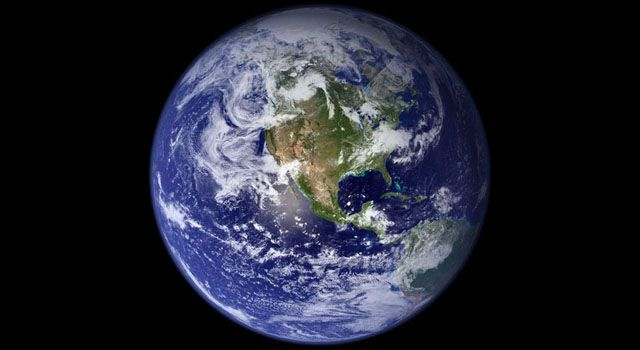
\includegraphics[width=0.4\textwidth]{earth}
		\hspace{2cm}
		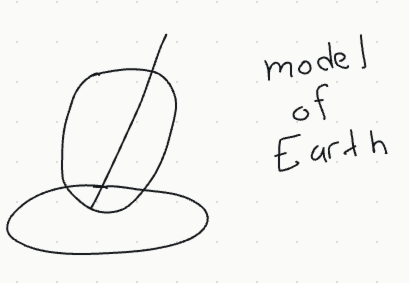
\includegraphics[width=0.4\textwidth]{model-of-earth}
		\caption{The Earth and a model of the earth (\href{https://www.space.com/54-earth-history-composition-and-atmosphere.html}{image by NASA)}}
		\label{fig:earth-model}
	\end{figure}
	The goals of models are:
	\begin{enumerate}[label=(\arabic*)]
		\item \textbf{Predictions}: This is the goal of this class.
		\item \textbf{Explanation}: This is the focus of other courses such has MATH 343.
	\end{enumerate}
	In \textbf{reality}, we can perform \textbf{measurements} if we have the right tools, and
	we will obtain \textbf{data} (see Figure~\ref{fig:data}).
	\begin{figure}
		\centering
		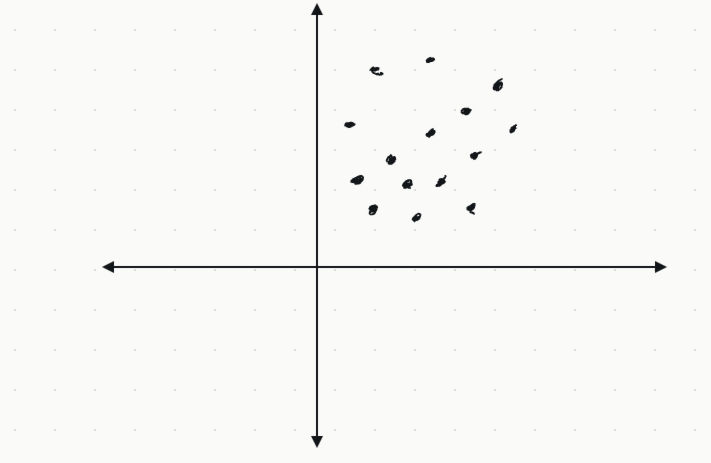
\includegraphics[width=0.4\textwidth]{data}
		\caption{Data measurements in some phenomenon.}
		\label{fig:data}
	\end{figure}
	From the model, you can make \textbf{predictions} (see Figure~\ref{fig:predictions}).
	\begin{figure}
		\centering
		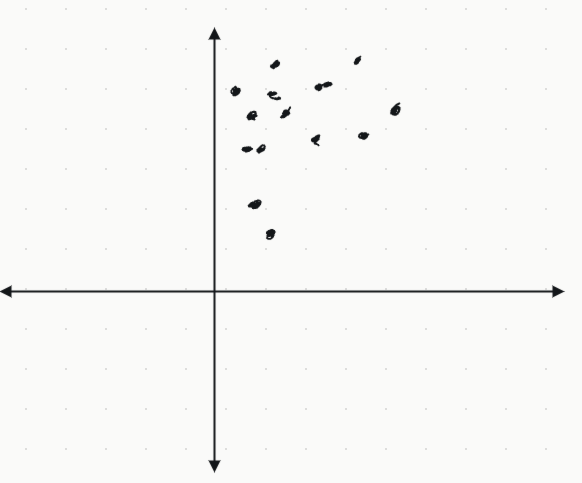
\includegraphics[width=0.4\textwidth]{predictions}
		\caption{Predictions based on model to some phenomenon.}
		\label{fig:predictions}
	\end{figure}
	A natural question is: are our predictions \textbf{accurate}? To determine this, we compare
	the predictions to the data that we gathered and we perform \textbf{validation}.
	However, a very important fact to remember is that \textit{predictions are not reality}!
	Data is the result of a system phenomenon in reality. If the predictions are close to it,
	then we have done well.
	
	Consider again the quote on human success. We can think of it as as a function:
	\begin{align*}
		\begin{bmatrix}
			\text{health}\\
			\text{wealth}\\
			\text{wisdom}
		\end{bmatrix}
		=
		f\left(\begin{bmatrix}
			\text{bedtime}\\
			\text{waketime}
		\end{bmatrix}\right)
	\end{align*}
	For now, we will say $f$ is \textbf{deterministic}. A problem with the formulation above
	is the fact that the english language is ambiguous. Bedtime is ill-defined, as well as
	health, wisdom, wealth, and waketime. THe model from the quote does not tell us how to measure
	the inputs or outputs.
	
	How can we make this model exact? We need a \textbf{metric}, i.e., a way to exactly,
	unambiguously numerically measure all inputs and outputs. For this model, we need 5 metrics:
	\begin{enumerate}[label=(\arabic*)]
		\item \textbf{Bedtime}: Perhaps we can say seconds, average all bedtimes
		since some age, such as 22.
		\item \textbf{Waketime}: We can use a similar metric as bedtime.
		\item \textbf{Health}: Medical literature invented a quality-of-life metric that we can use.
		\item \textbf{Wealth}: Maybe your net worth, or rate of change of your financial state.
		\item \textbf{Wisdom}: Maybe the number of books you have read.
	\end{enumerate}
	As you can see, coming up with metrics is difficult. Nevertheless, once you have defined metrics,
	these become scalars, and we can get on to modeling. What we do learn from this model
	is that it is not very operational. We don't say ``bad", however, because it is not
	``bad" until we use it to make predictions.
	
	\textbf{Mathematical models} are a subset of all models. Mathematical models will be the
	focus of this course because they are ambiguous. Mathematical models go back to
	about 2000 BCE. When you do science, you are building models, and we have built amazingly
	accurate mathematical models, such as:
	\begin{align*}
		F=ma\quad\implies\quad a=\frac{F}{m}
	\end{align*}
	This model uses the mass of an object and the force applied to it as inputs, and computes
	the acceleration of the object as an output. Another famous model is $E=mc^2$.
	The universe is explicable mathematically, regardless of whether you believe it.
	For the purposes of this class:
	\begin{itemize}
		\item Phenomena \textit{are} explicable mathematically.
		\item One output for the functions in our models.
	\end{itemize}
	We will often use the following notation:
	\begin{align*}
		y = t(z_1,z_2,\ldots,z_t)
	\end{align*}
	Their meaning is:
	\begin{itemize}
		\item $z_1,z_2,\ldots,z_t$ are the true, causal input information.
		\item $y$ is the output, phenomenon, response, outcome, or dependent variable.
		\item $t$ is the exact functional relationship.
	\end{itemize}
	%\pagebreak
	%\printbibliography
\end{document}